\newif\ifteacher\teacherfalse
\documentclass[11pt,a4paper]{article}
\usepackage[margin=2.4cm,top=2.2cm]{geometry}
\usepackage{amsmath,amssymb}
\usepackage{tgschola}\usepackage{fouriernc}
\linespread{1.05}
\usepackage[T1]{fontenc}
\usepackage{microtype}
\usepackage{tikz}
\usetikzlibrary{angles,quotes,calc,arrows.meta}
\usepackage{enumitem}
\usepackage{needspace}
\usepackage{tfrupee}
\definecolor{figline}{RGB}{64,64,64}
\definecolor{figfill}{RGB}{232,232,232}
\definecolor{figfill2}{RGB}{214,214,214}
\definecolor{muted}{RGB}{72,74,78}
\definecolor{thinrule}{RGB}{128,128,128}
\pagestyle{plain}
\setlength{\parindent}{0pt}
\setlength{\parskip}{1pt}
\setlength{\lineskiplimit}{2pt}\setlength{\lineskip}{4pt}
\setlength{\emergencystretch}{2em}
\tikzset{fig/.style={draw=figline}}
\newcommand{\nl}{\\[3pt]}
\newcounter{qn}
\newcommand{\ques}{\par\medskip\refstepcounter{qn}\noindent\hangindent=1.7em\hangafter=1\makebox[1.7em][l]{\textbf{\arabic{qn}.}}\ignorespaces}
\newcommand{\pc}[2]{\par\smallskip\noindent\hspace*{2em}\hangindent=4.3em\hangafter=1\makebox[2em][l]{(#1)}\hspace{0.3em}#2\par}
\newcommand{\mcqone}[4]{\par\smallskip\noindent\hspace*{2em}\hangindent=4.3em\hangafter=1(a)~#1 \qquad (b)~#2 \qquad (c)~#3 \qquad (d)~#4\par}
\newcommand{\mcqtwo}[4]{\par\smallskip\noindent\hspace*{2em}\begin{tabular}[t]{@{}p{0.42\linewidth}@{\hspace{1.6em}}p{0.42\linewidth}@{}}(a)~#1 & (b)~#2 \\[5pt](c)~#3 & (d)~#4\end{tabular}\par\smallskip}
\newcommand{\optline}[1]{\par\vspace{2pt}\noindent\hspace*{2em}\hangindent=4.3em\hangafter=1 #1}
\newcommand{\aritem}[2]{\par\smallskip\noindent\hspace*{1.7em}\hangindent=1.7em\hangafter=1 #1:~#2\par}
\newcommand{\orline}{\par\smallskip{\centering\textit{OR}\par}\nopagebreak\smallskip}
\newcommand{\sect}[1]{\par\medskip\Needspace{15\baselineskip}{\small\bfseries #1}\par\nopagebreak\smallskip}
\ifteacher
\newenvironment{answerblock}
  {\par\needspace{6\baselineskip}\smallskip\begingroup\small\linespread{1.2}\selectfont\color{muted}\noindent\textit{Answer.}\par}
  {\par\endgroup\medskip}
\newcommand{\ap}[1]{\par\smallskip\noindent\textbf{(#1)}\ }
\else
\usepackage{comment}
\excludecomment{answerblock}
\fi
\makeatletter
\newcommand{\figslot}[1]{\@ifundefined{fig@#1}{}{\csname fig@#1\endcsname}}
\makeatother

\begin{document}
\noindent{\large\bfseries Practice questions}\hfill 28 October 2026\par
\vspace{2pt}
\noindent\rule{\linewidth}{0.6pt}\par
\vspace{2pt}
{\small Use $\pi=\dfrac{22}{7}$. For every question without a picture, first draw a rough diagram and mark all the given measurements on it. Show all your steps.\par}
\ifteacher
\vspace{4pt}
{\color{thinrule}\noindent\rule{\linewidth}{0.4pt}}\par
\vspace{4pt}
{\small\color{muted}\linespread{1.15}\selectfont
\textbf{Purpose.} This set revises the whole chapter. The questions follow the style of the NCERT textbook \textit{Ganita Manjari}, Grade~9, Chapter~6. They go from easier to harder.\nl
\textbf{Competency focus.} Students work backwards from a result, find and explain a mistake, test a claim, compare two methods, and apply results to real situations. Several questions ask students to draw a diagram.\nl
\textbf{Concepts assessed.} Circumference of a circle (Q1, 12); the number $\pi$ (Q2); arc length (Q3, 13); the stagger on a running track (Q4); area of a parallelogram (Q5, 7); area of a triangle and triangles between the same parallels (Q6); the median of a triangle (Q7); Heron's formula (Q8, 9); Brahmagupta's formula (Q10); Baudh\={a}yana's method of squaring a rectangle (Q11); area of a circle (Q12, 15); area of a sector and a ring sector (Q13); area of a segment (Q14); composite figures (Q15).\nl
\textbf{Answers.} Answers appear in grey after each question, with a rough answer diagram.\par}
\vspace{4pt}
{\color{thinrule}\noindent\rule{\linewidth}{0.4pt}}\par
\vspace{3pt}
\fi
\Needspace{8\baselineskip}
\ques A circular lotus pond in a temple garden is fenced once with $132$~m of wire. Draw a rough diagram.\par
\pc{a}{Find the radius of the pond.}
\pc{b}{A second fence is put up $7$~m outside the first fence, all the way round. Find how much more wire the second fence needs than the first.}
\pc{c}{Another pond has a radius of $35$~m. It also gets a second fence $7$~m outside the first one. Will the extra wire needed be more than, less than, or the same as your answer to (b)? Explain.}
\begin{answerblock}
\ap{a} The wire is the circumference of the pond, so $2\times\dfrac{22}{7}\times r=132$.\nl
Therefore $r=132\times\dfrac{7}{2\times22}=21$. The radius of the pond is $21$~m.\nl
\ap{b} The second fence has radius $21+7=28$~m, so its circumference is $2\times\dfrac{22}{7}\times28=176$~m.\nl
The extra wire is $176-132=44$~m.\nl
\ap{c} The extra wire is the same, $44$~m. For any radius $R$ the extra is $2\times\dfrac{22}{7}\times(R+7)-2\times\dfrac{22}{7}\times R=2\times\dfrac{22}{7}\times7=44$~m.\nl
Check with $R=35$: $2\times\dfrac{22}{7}\times42-2\times\dfrac{22}{7}\times35=264-220=44$~m.
\begin{center}
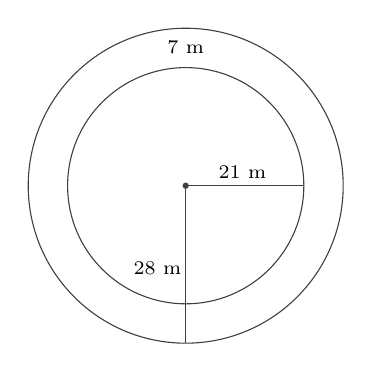
\begin{tikzpicture}[fig,every node/.style={font=\scriptsize}]
\draw[fig] (0,0) circle (2);
\draw[fig] (0,0) circle (1.5);
\draw[fig] (0,0) -- (1.5,0);
\draw[fig] (0,0) -- (0,-2);
\fill[figline] (0,0) circle (0.04);
\node at (0.72,0.17) {$21$~m};
\node at (-0.36,-1.05) {$28$~m};
\node at (0,1.76) {$7$~m};
\end{tikzpicture}
\end{center}
\end{answerblock}

\Needspace{8\baselineskip}
\ques Say whether each statement is true or false. Give a reason for each answer.\par
\pc{a}{The value of $\pi$ is exactly $\dfrac{22}{7}$.}
\pc{b}{For every circle, the circumference divided by the diameter gives the same number.}
\pc{c}{Arjun measures a bangle. Its circumference is $22$~cm and its diameter is $7$~cm. Arjun says, ``This proves that $\pi$ is exactly $\dfrac{22}{7}$.''}
\begin{answerblock}
\ap{a} False. $\pi$ is irrational, so no fraction of two whole numbers equals it.\nl
$\dfrac{22}{7}=3.142\ldots$ and $\pi=3.14159\ldots$, so $\dfrac{22}{7}$ is only a close approximation.\nl
\ap{b} True. This constant ratio is the same for every circle, and it is the number $\pi$.\nl
\ap{c} False. Every measurement is approximate, so a measurement cannot prove an exact value.\nl
Also $\pi$ is irrational, so $\pi$ cannot equal $\dfrac{22}{7}$.
\begin{center}
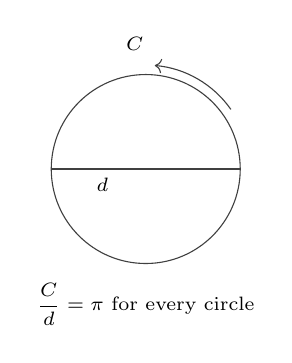
\begin{tikzpicture}[fig,every node/.style={font=\scriptsize}]
\draw[fig] (0,0) circle (1.2);
\draw[fig] (-1.2,0) -- (1.2,0);
\draw[fig,->] (35:1.32) arc (35:85:1.32);
\node at (-0.55,-0.2) {$d$};
\node at (95:1.6) {$C$};
\node at (0,-1.72) {$\dfrac{C}{d}=\pi$ for every circle};
\end{tikzpicture}
\end{center}
\end{answerblock}

\Needspace{8\baselineskip}
\ques A railway line goes round a curve. The curve is an arc of a circle of radius $210$~m.\par
\pc{a}{A train goes round the curve and turns through an angle of $60^\circ$. Draw a rough diagram. Find the distance the train travels on the curve.}
\pc{b}{On another curve of the same radius, a train travels $330$~m. Find the angle through which the train turns.}
\begin{answerblock}
\ap{a} The diagram below shows the arc, its radius and the angle at the centre.\nl
The arc is the fraction $\dfrac{60}{360}=\dfrac16$ of the whole circle.\nl
Arc $=\dfrac{60}{360}\times2\times\dfrac{22}{7}\times210=\dfrac16\times1320=220$~m. The train travels $220$~m.\nl
\ap{b} The whole circumference is $2\times\dfrac{22}{7}\times210=1320$~m.\nl
The arc is $\dfrac{330}{1320}=\dfrac14$ of the circle, so the angle is $\dfrac14\times360=90^\circ$.
\begin{center}
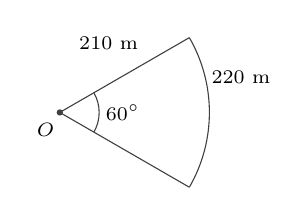
\begin{tikzpicture}[fig,every node/.style={font=\scriptsize}]
\draw[fig] (0,0) -- (30:1.9);
\draw[fig] (0,0) -- (-30:1.9);
\draw[fig] (30:1.9) arc (30:-30:1.9);
\draw[fig] (30:0.5) arc (30:-30:0.5);
\fill[figline] (0,0) circle (0.04);
\node at (-0.18,-0.22) {$O$};
\node at (0.62,0.88) {$210$~m};
\node at (0.8,0) {$60^\circ$};
\node at (2.3,0.45) {$220$~m};
\end{tikzpicture}
\end{center}
\end{answerblock}

\Needspace{8\baselineskip}
\ques In a $200$~m race on a school track, each runner runs one bend and one straight. The bend in every lane is a semicircle. Each lane is $1.4$~m wide. All runners finish at the same line. Assume that each runner runs along the inner edge of the lane. Draw a rough diagram of lanes 1 and 2.\par
\pc{a}{Explain why the runner in lane 2 must start ahead of the runner in lane 1.}
\pc{b}{Find how far ahead of the lane 1 runner the lane 2 runner must start.}
\pc{c}{Find how far ahead of the lane 1 runner the lane 4 runner must start.}
\pc{d}{Ravi says, ``If the track had a bigger bend, the answer to (b) would change.'' Is Ravi right? Explain.}
\begin{answerblock}
\ap{a} The two straights are equal, but the bend in lane 2 has the larger radius, so it is longer.\nl
Therefore the lane 2 runner starts ahead, so that every runner covers $200$~m.\nl
\ap{b} The radius of the lane 2 bend is $r+1.4$, so the extra length is $\dfrac{22}{7}\times(r+1.4)-\dfrac{22}{7}\times r=\dfrac{22}{7}\times1.4=4.4$~m.\nl
The lane 2 runner starts $4.4$~m ahead of the lane 1 runner.\nl
\ap{c} The lane 4 bend has radius $r+3\times1.4=r+4.2$, so the extra length is $\dfrac{22}{7}\times4.2=13.2$~m, which is $3\times4.4$~m.\nl
The lane 4 runner starts $13.2$~m ahead of the lane 1 runner.\nl
\ap{d} No. The difference is $\dfrac{22}{7}\times1.4=4.4$~m, and the radius $r$ cancels from the subtraction.\nl
So the stagger does not depend on the size of the bend, and Ravi is wrong.
\begin{center}
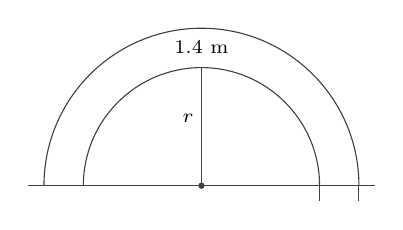
\begin{tikzpicture}[fig,every node/.style={font=\scriptsize}]
\draw[fig] (-2.2,0) -- (2.2,0);
\draw[fig] (1.5,0) arc (0:180:1.5);
\draw[fig] (2,0) arc (0:180:2);
\draw[fig] (0,0) -- (0,1.5);
\draw[fig] (1.5,0) -- (1.5,-0.2);
\draw[fig] (2,0) -- (2,-0.2);
\fill[figline] (0,0) circle (0.04);
\node at (-0.17,0.85) {$r$};
\node at (0,1.76) {$1.4$~m};
\end{tikzpicture}
\end{center}
\end{answerblock}

\Needspace{8\baselineskip}
\ques A garden bed ABCD is shaped like a parallelogram. AB $=18$~m and AD $=12$~m. The perpendicular distance between the sides AB and DC is $10$~m.\par
\pc{a}{Draw a rough diagram. Mark all the lengths and show the $10$~m distance with a dotted line.}
\pc{b}{Raju finds the area like this: Area $=18\times12=216$~m$^2$. Explain Raju's mistake. Find the correct area of the bed.}
\pc{c}{Find the perpendicular distance between the sides AD and BC.}
\begin{answerblock}
\ap{a} See the diagram below. The base $AB=18$~m and the slanting side $AD=12$~m are marked, and the height of $10$~m on $AB$ is drawn dotted.\nl
\ap{b} Raju multiplied the two sides. The area of a parallelogram is base $\times$ perpendicular height on that base, and $12$~m is a slanting side, not the height on $AB$.\nl
Area $=18\times10=180$~m$^2$.\nl
\ap{c} The area also equals $AD\times$ the perpendicular height on $AD$, so $12\times h=180$.\nl
Therefore $h=15$~m. The distance between $AD$ and $BC$ is $15$~m.
\begin{center}
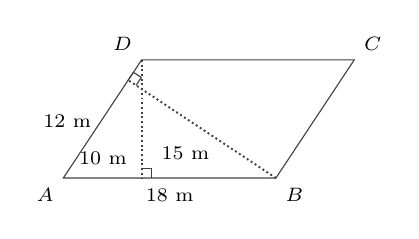
\begin{tikzpicture}[fig,every node/.style={font=\scriptsize}]
\draw[fig] (0,0) -- (2.7,0) -- (3.6945,1.5) -- (0.9945,1.5) -- cycle;
\draw[fig,densely dotted,line width=0.7pt] (0.9945,1.5) -- (0.9945,0);
\draw[fig,densely dotted,line width=0.7pt] (2.7,0) -- (0.824,1.243);
\draw[fig] (1.1145,0) -- (1.1145,0.12) -- (0.9945,0.12);
\draw[fig] (0.824,1.243) -- (0.890,1.343) -- (0.990,1.277) -- (0.924,1.177);
\node at (1.35,-0.22) {$18$~m};
\node at (0.05,0.72) {$12$~m};
\node[left] at (0.93,0.25) {$10$~m};
\node at (1.55,0.32) {$15$~m};
\node[below left] at (0,0) {$A$};
\node[below right] at (2.7,0) {$B$};
\node[above right] at (3.6945,1.5) {$C$};
\node[above left] at (0.9945,1.5) {$D$};
\end{tikzpicture}
\end{center}
\end{answerblock}
\Needspace{8\baselineskip}
\ques A strip of cloth has two straight parallel edges that are $7$~cm apart. Kavi draws two triangles, $PQR$ and $SQR$, on the strip. Both triangles have the side $QR=12$~cm along the lower edge. The points $P$ and $S$ are on the upper edge. In triangle $PQR$, the angles at $Q$ and $R$ are acute. In triangle $SQR$, the angle at $Q$ is obtuse.\par
\pc{a}{Draw both triangles in one rough diagram. Show the height of each triangle with a dotted line.}
\pc{b}{Find the area of each triangle.}
\pc{c}{Priya says, ``Triangle $SQR$ has the larger area, because its sides are longer.'' Is Priya right? Explain.}
\begin{answerblock}
\ap{a} See the diagram.
\ap{b} Each triangle has base $QR=12$~cm and height $7$~cm, the distance between the parallel edges.\nl
Area $=\dfrac12\times12\times7=42$~cm$^2$ each.\nl
For $SQR$ the height falls outside the triangle, on $RQ$ extended, but it is still $7$~cm.
\ap{c} No. The area depends on the base and the perpendicular height, not on the slanting sides.\nl
Both triangles have base $12$~cm and height $7$~cm, so both areas are $42$~cm$^2$.
\begin{center}
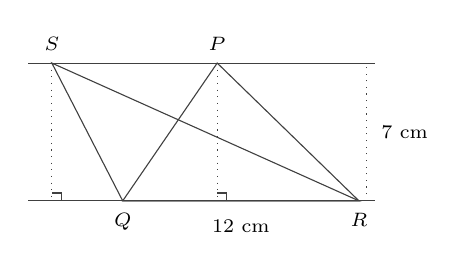
\begin{tikzpicture}[fig,every node/.style={font=\scriptsize}]
\draw[fig] (-1.2,0) -- (3.2,0);
\draw[fig] (-1.2,1.75) -- (3.2,1.75);
\draw[fig] (1.2,1.75) -- (0,0) -- (3.0,0) -- cycle;
\draw[fig] (-0.9,1.75) -- (0,0) -- (3.0,0) -- cycle;
\draw[fig,dotted] (-0.9,1.75) -- (-0.9,0);
\draw[fig,dotted] (1.2,1.75) -- (1.2,0);
\draw[fig] (-0.9,0.1) -- (-0.78,0.1) -- (-0.78,0);
\draw[fig] (1.2,0.1) -- (1.32,0.1) -- (1.32,0);
\draw[fig,dotted] (3.1,0) -- (3.1,1.75);
\node[above] at (1.2,1.79) {$P$};
\node[above] at (-0.9,1.79) {$S$};
\node[below] at (0,-0.03) {$Q$};
\node[below] at (3.0,-0.03) {$R$};
\node[below] at (1.5,-0.12) {$12$~cm};
\node[right] at (3.16,0.875) {$7$~cm};
\end{tikzpicture}
\end{center}
\end{answerblock}

\Needspace{8\baselineskip}
\ques A glass panel $ABCD$ in a lamp is shaped like a parallelogram, and its area is $96$~cm$^2$. Two thin metal strips run along the diagonals $AC$ and $BD$. They meet at $O$ and divide the glass into four triangular pieces. Draw a rough diagram.\par
\pc{a}{Explain why triangles $AOB$ and $BOC$ have equal areas. (Hint: what is $BO$ in triangle $ABC$?)}
\pc{b}{Explain why all four pieces have equal areas. Find the area of each piece.}
\pc{c}{Neha says, ``The four pieces are congruent.'' Is Neha right? Explain.}
\begin{answerblock}
\ap{a} The diagonals of a parallelogram bisect each other, so $O$ is the midpoint of $AC$.\nl
So $BO$ is a median of triangle $ABC$. A median divides a triangle into two triangles of equal area, so the area of $AOB$ equals the area of $BOC$.
\ap{b} In the same way, $CO$ is a median of triangle $BCD$ ($O$ is the midpoint of $BD$), so the area of $BOC$ equals the area of $COD$; and $DO$ is a median of triangle $CDA$, so the area of $COD$ equals the area of $DOA$.\nl
So all four pieces are equal. Each $=96\div4=24$~cm$^2$.
\ap{c} Not in general. $AOB$ is congruent to $COD$, and $BOC$ is congruent to $DOA$ (SAS: $OA=OC$, $OB=OD$, vertically opposite angles).\nl
But $AOB$ and $BOC$ have different sides when $AB\ne BC$, so they are not congruent.\nl
They are all congruent only when $ABCD$ is a rhombus. Equal area does not mean congruent.
\begin{center}
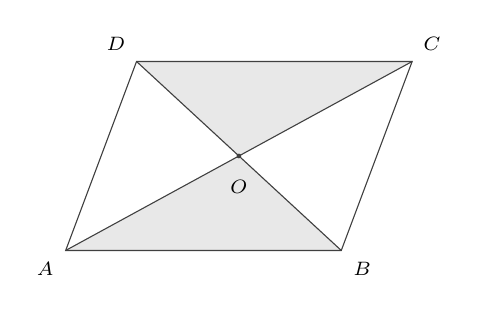
\begin{tikzpicture}[fig,every node/.style={font=\scriptsize}]
\fill[figfill] (0,0) -- (3.5,0) -- (2.2,1.2) -- cycle;
\fill[figfill] (4.4,2.4) -- (0.9,2.4) -- (2.2,1.2) -- cycle;
\draw[fig] (0,0) -- (3.5,0) -- (4.4,2.4) -- (0.9,2.4) -- cycle;
\draw[fig] (0,0) -- (4.4,2.4);
\draw[fig] (3.5,0) -- (0.9,2.4);
\fill[figline] (2.2,1.2) circle (0.03);
\node[below] at (2.2,1.02) {$O$};
\node[below left] at (-0.03,-0.02) {$A$};
\node[below right] at (3.53,-0.02) {$B$};
\node[above right] at (4.42,2.42) {$C$};
\node[above left] at (0.88,2.42) {$D$};
\end{tikzpicture}
\end{center}
\end{answerblock}

\Needspace{8\baselineskip}
\ques A triangular plot $ABC$ has sides $BC=90$~m, $CA=100$~m and $AB=170$~m.\par
\pc{a}{Find the area of the plot using Heron's formula.}
\pc{b}{Use your answer to (a) to find the shortest distance from the corner $A$ to the line $BC$.}
\pc{c}{Draw a rough diagram showing this shortest distance $AD$. Does $D$ lie on the side $BC$, or on $BC$ extended beyond $C$? Find $CD$ and check your answer to (b) using $AB$.}
\begin{answerblock}
\ap{a} $s=\dfrac{90+100+170}{2}=180$. $s-a=90$, $s-b=80$, $s-c=10$.\nl
Area $=\sqrt{180\times90\times80\times10}=\sqrt{12960000}=3600$~m$^2$.
\ap{b} $\dfrac12\times90\times AD=3600$, so $AD=80$~m.
\ap{c} Angle $C$ is obtuse, so $D$ lies on $BC$ extended beyond $C$.\nl
In right triangle $ADC$: $CD=\sqrt{100^2-80^2}=\sqrt{3600}=60$~m. $BD=90+60=150$~m.\nl
In right triangle $ADB$: $AB=\sqrt{150^2+80^2}=\sqrt{28900}=170$~m.\nl
This matches, so $AD=80$~m is correct.
\begin{center}
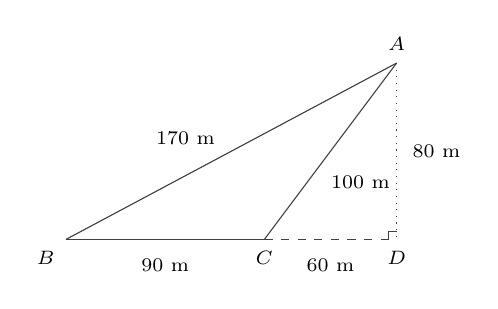
\begin{tikzpicture}[fig,every node/.style={font=\scriptsize}]
\draw[fig] (0,0) -- (2.52,0);
\draw[fig,dashed] (2.52,0) -- (4.2,0);
\draw[fig] (4.2,2.24) -- (0,0);
\draw[fig] (4.2,2.24) -- (2.52,0);
\draw[fig,dotted] (4.2,2.24) -- (4.2,0);
\draw[fig] (4.1,0) -- (4.1,0.1) -- (4.2,0.1);
\node[below left] at (-0.02,-0.02) {$B$};
\node[below] at (2.52,-0.03) {$C$};
\node[below] at (4.2,-0.03) {$D$};
\node[above] at (4.2,2.28) {$A$};
\node[below] at (1.26,-0.12) {$90$~m};
\node[below] at (3.36,-0.12) {$60$~m};
\node[left] at (2.015,1.28) {$170$~m};
\node at (3.74,0.72) {$100$~m};
\node[right] at (4.28,1.12) {$80$~m};
\end{tikzpicture}
\end{center}
\end{answerblock}

\Needspace{8\baselineskip}
\ques A garden bed is shaped like an isosceles triangle. Its perimeter is $64$~m and its unequal side (the base) is $24$~m. Draw a rough diagram.\par
\pc{a}{Find the length of each equal side.}
\pc{b}{Find the area of the bed using Heron's formula.}
\pc{c}{Find the area again in a different way, using the height on the base. Check that both answers agree.}
\begin{answerblock}
\ap{a} $(64-24)\div2=20$~m.
\ap{b} $s=32$; $s-a=12$, $s-b=12$, $s-c=8$.\nl
Area $=\sqrt{32\times12\times12\times8}=\sqrt{36864}=192$~m$^2$.
\ap{c} The height from the top corner meets the base at its midpoint, $12$~m from each end.\nl
Height $=\sqrt{20^2-12^2}=\sqrt{256}=16$~m. Area $=\dfrac12\times24\times16=192$~m$^2$.\nl
Both answers agree.
\begin{center}
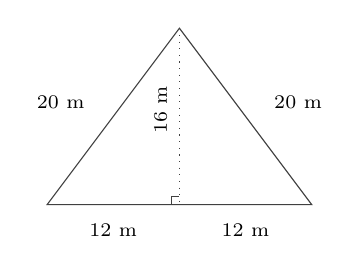
\begin{tikzpicture}[fig,every node/.style={font=\scriptsize}]
\draw[fig] (0,0) -- (3.36,0) -- (1.68,2.24) -- cycle;
\draw[fig,dotted] (1.68,2.24) -- (1.68,0);
\draw[fig] (1.58,0) -- (1.58,0.1) -- (1.68,0.1);
\node[left] at (0.60,1.30) {$20$~m};
\node[right] at (2.76,1.30) {$20$~m};
\node[rotate=90] at (1.44,1.2) {$16$~m};
\node[below] at (0.84,-0.12) {$12$~m};
\node[below] at (2.52,-0.12) {$12$~m};
\end{tikzpicture}
\end{center}
\end{answerblock}

\Needspace{8\baselineskip}
\ques A plot of land $ABCD$ has all four corners on a circle, as shown. $AB=25$~m, $BC=60$~m, $CD=52$~m and $DA=39$~m.\par
\pc{a}{Find the area of the plot using Brahmagupta's formula.}
\pc{b}{The diagonal $AC$ is a diameter of the circle, and $AC=65$~m. So the angles at $B$ and $D$ are right angles. Find the area of the plot again by splitting it along $AC$ into two triangles. Check that it agrees with (a).}
\pc{c}{A rectangle $12$~m by $5$~m also has all four corners on a circle. Use Brahmagupta's formula to find its area. Does the formula give the answer you expect? Explain.}
\begin{center}
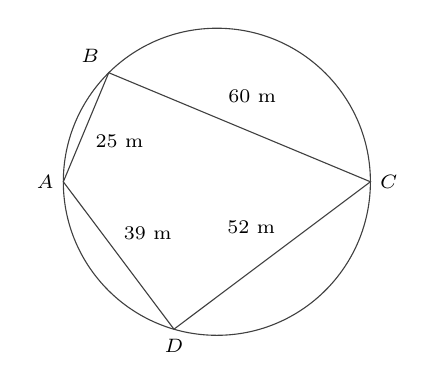
\begin{tikzpicture}[fig,every node/.style={font=\scriptsize}]
\draw[fig] (0,0) circle (1.95);
\draw[fig] (-1.95,0) -- (-1.373,1.385) -- (1.95,0) -- (-0.545,-1.872) -- cycle;
\node at (-1.237,0.515) {$25$~m};
\node at (0.450,1.080) {$60$~m};
\node at (0.437,-0.583) {$52$~m};
\node at (-0.879,-0.660) {$39$~m};
\node[left] at (-1.95,0) {$A$};\node[above left] at (-1.373,1.385) {$B$};\node[right] at (1.95,0) {$C$};\node[below] at (-0.545,-1.872) {$D$};
\end{tikzpicture}
\end{center}
\begin{answerblock}
\ap{a} $s=\dfrac{25+60+52+39}{2}=88$. $s-a=63$, $s-b=28$, $s-c=36$, $s-d=49$.\nl
Area $=\sqrt{63\times28\times36\times49}=\sqrt{3111696}=1764$~m$^2$.
\ap{b} Area of $ABC=\dfrac12\times25\times60=750$~m$^2$; area of $ACD=\dfrac12\times39\times52=1014$~m$^2$; total $=750+1014=1764$~m$^2$.\nl
This agrees with (a).
\ap{c} $s=\dfrac{12+5+12+5}{2}=17$; $(17-12)(17-5)(17-12)(17-5)=5\times12\times5\times12=3600$; area $=\sqrt{3600}=60$~m$^2=12\times5$.\nl
Yes: for a rectangle the formula gives $\sqrt{b\times l\times b\times l}=l\times b$, the correct area.
\begin{center}
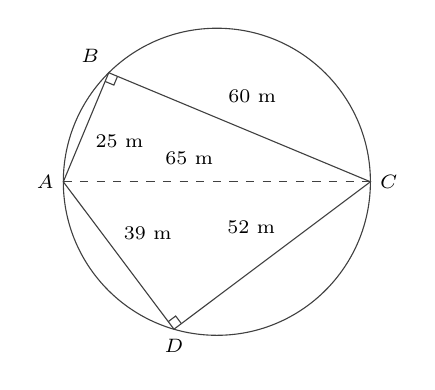
\begin{tikzpicture}[fig,every node/.style={font=\scriptsize}]
\draw[fig] (0,0) circle (1.95);
\draw[fig,dashed] (-1.95,0) -- (1.95,0);
\draw[fig] (-1.95,0) -- (-1.373,1.385) -- (1.95,0) -- (-0.545,-1.872) -- cycle;
\draw[fig] (-1.419,1.274) -- (-1.308,1.228) -- (-1.262,1.339);
\draw[fig] (-0.451,-1.801) -- (-0.523,-1.705) -- (-0.617,-1.776);
\node at (-1.237,0.515) {$25$~m};
\node at (0.450,1.080) {$60$~m};
\node at (0.437,-0.583) {$52$~m};
\node at (-0.879,-0.660) {$39$~m};
\node[left] at (-1.95,0) {$A$};\node[above left] at (-1.373,1.385) {$B$};\node[right] at (1.95,0) {$C$};\node[below] at (-0.545,-1.872) {$D$};
\node at (-0.35,0.30) {$65$~m};
\end{tikzpicture}
\end{center}
\end{answerblock}
\Needspace{13\baselineskip}
\ques Long ago, Baudh\={a}yana showed how to change a rectangle into a square of the same area. Follow his steps for a rectangular field $18$~m long and $8$~m wide. Draw a diagram for each step.\par
\pc{a}{Cut off a square of side $8$~m from one end of the rectangle. What are the length and breadth of the strip that is left?}
\pc{b}{Cut the strip into two equal strips, each $8$~m long. Place one strip along the right side of the square and the other along the top of the square. This makes an L-shape. Show that the L-shape fits inside a square of side $13$~m, with a small square missing at one corner. Find the side of the missing square.}
\pc{c}{Find the area of the L-shape in two ways: from the rectangle, and as (big square) $-$ (small square).}
\pc{d}{Baudh\={a}yana now draws a right triangle with hypotenuse $13$~m and one side $5$~m. Find the third side. Explain why a square on this third side has the same area as the field.}
\begin{answerblock}
\ap{a} The square cut off has side $8$~m, so the strip left is $18-8=10$~m long and $8$~m broad.\nl
Its area is $10\times8=80$~m$^2$.
\ap{b} Each new strip is $5$~m by $8$~m, because the $10$~m side of the strip is cut in half.\nl
The square then measures $8+5=13$~m along each side, except at the corner where a $5$~m by $5$~m square is empty.\nl
So the side of the missing square is $5$~m.
\ap{c} From the rectangle: $18\times8=144$~m$^2$.\nl
From the squares: $13^2-5^2=169-25=144$~m$^2$. Both methods give $144$~m$^2$.
\ap{d} The third side is $\sqrt{13^2-5^2}=\sqrt{144}=12$~m.\nl
By Pythagoras, the square on this side has area $12^2=144$~m$^2$, and $13^2-5^2$ is also the area of the L-shape, which equals the area of the field.
\begin{center}
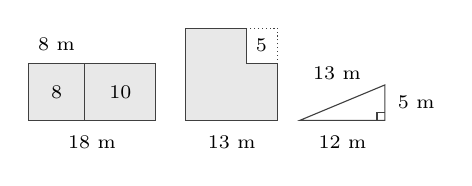
\begin{tikzpicture}[fig,every node/.style={font=\scriptsize}]
\fill[figfill] (0,0) rectangle (1.62,0.72);
\draw[fig] (0,0) rectangle (1.62,0.72);
\draw[fig] (0.72,0) -- (0.72,0.72);
\node at (0.36,0.36) {$8$};
\node at (1.17,0.36) {$10$};
\node[below] at (0.81,-0.07) {$18$~m};
\node[above] at (0.36,0.76) {$8$~m};
\fill[figfill] (2.00,0) -- (3.17,0) -- (3.17,0.72) -- (2.77,0.72) -- (2.77,1.17) -- (2.00,1.17) -- cycle;
\draw[fig] (2.00,0) -- (3.17,0) -- (3.17,0.72) -- (2.77,0.72) -- (2.77,1.17) -- (2.00,1.17) -- cycle;
\draw[fig,densely dotted] (3.17,0.72) -- (3.17,1.17) -- (2.77,1.17);
\node[inner sep=0.5pt] at (2.96,0.95) {$5$};
\node[below] at (2.585,-0.07) {$13$~m};
\draw[fig] (3.45,0) -- (4.53,0) -- (4.53,0.45) -- cycle;
\draw[fig] (4.43,0) -- (4.43,0.10) -- (4.53,0.10);
\node[below] at (3.99,-0.07) {$12$~m};
\node[right] at (4.57,0.225) {$5$~m};
\node[above] at (3.92,0.40) {$13$~m};
\end{tikzpicture}
\end{center}
\end{answerblock}

\Needspace{9\baselineskip}
\ques The top of a round table has a circumference of $220$~cm.\par
\pc{a}{Find the radius of the table top.}
\pc{b}{Find the area of the table top.}
\pc{c}{A bigger round table has a radius twice as long. Ravi says, ``Its top has twice the area.'' Is Ravi right? Find the area of the bigger table top and explain.}
\begin{answerblock}
\ap{a} $2\times\dfrac{22}{7}\times r=220$, so $r=220\times\dfrac{7}{22}\times\dfrac12=35$~cm.
\ap{b} Area $=\dfrac{22}{7}\times35\times35=3850$~cm$^2$.
\ap{c} No. The new radius is $70$~cm, so its area is $\dfrac{22}{7}\times70\times70=15400$~cm$^2$, which is $4\times3850$~cm$^2$.\nl
When the radius doubles, $r\times r$ becomes four times as large, so the area becomes four times as large, not twice.
\begin{center}
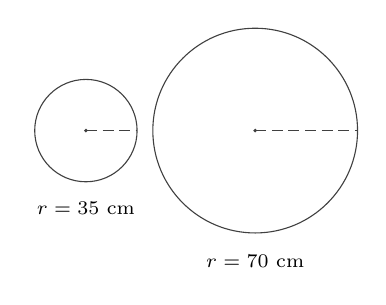
\begin{tikzpicture}[fig,every node/.style={font=\scriptsize}]
\draw[fig] (0,0) circle (0.65);
\draw[fig,dash pattern=on 4pt off 2pt] (0,0) -- (0.65,0);
\fill[figline] (0,0) circle (0.025);
\node[below] at (0,-0.78) {$r=35$~cm};
\draw[fig] (2.15,0) circle (1.30);
\draw[fig,dash pattern=on 4pt off 2pt] (2.15,0) -- (3.45,0);
\fill[figline] (2.15,0) circle (0.025);
\node[below] at (2.15,-1.46) {$r=70$~cm};
\end{tikzpicture}
\end{center}
\end{answerblock}

\Needspace{9\baselineskip}
\ques A car's wiper arm is $21$~cm long and turns about one end, $O$. The rubber blade is fixed to the outer part of the arm, from $7$~cm to $21$~cm from $O$. The arm turns through an angle of $90^\circ$.\par
\pc{a}{Draw a rough diagram. Shade the part of the glass that the blade wipes.}
\pc{b}{Find the area of the glass that the blade wipes.}
\pc{c}{Find the length of the path of the tip of the arm.}
\begin{answerblock}
\ap{a} See the diagram.
\ap{b} The wiped part is the difference of two sectors of angle $90^\circ$, with radii $21$~cm and $7$~cm.\nl
Area $=\dfrac{90}{360}\times\dfrac{22}{7}\times(21\times21-7\times7)=\dfrac14\times\dfrac{22}{7}\times392=308$~cm$^2$.
\ap{c} The tip moves along an arc of radius $21$~cm.\nl
Path $=\dfrac{90}{360}\times2\times\dfrac{22}{7}\times21=33$~cm.
\begin{center}
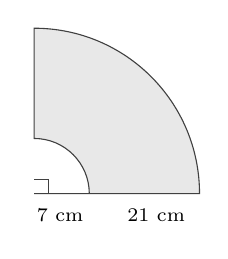
\begin{tikzpicture}[fig,every node/.style={font=\scriptsize}]
\fill[figfill] (0,0) -- (0.7,0) arc (0:90:0.7) -- (0,2.1) arc (90:0:2.1) -- cycle;
\draw[fig] (0,0) -- (0.7,0) arc (0:90:0.7) -- (0,2.1) arc (90:0:2.1) -- cycle;
\draw[fig] (0.18,0) -- (0.18,0.18) -- (0,0.18);
\node[below] at (0.33,-0.07) {$7$~cm};
\node[below] at (1.55,-0.07) {$21$~cm};
\end{tikzpicture}
\end{center}
\end{answerblock}

\Needspace{17\baselineskip}
\ques A floor tile $ABCD$ is a square of side $14$~cm. Two quarter circles are drawn inside it: one with centre $A$ and radius $AB$, and one with centre $C$ and radius $CB$. Both arcs go from $B$ to $D$. The leaf-shaped part between the two arcs is shaded.\par
\pc{a}{Find the area of the shaded leaf.}
\pc{b}{Find the perimeter of the shaded leaf.}
\pc{c}{Meena finds the area of the leaf like this: (area of one quarter circle) $+$ (area of the other quarter circle) $-$ (area of the square). Explain why her method works, and check that it gives the same answer.}
\begin{center}
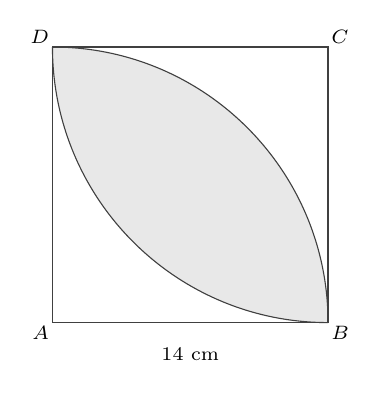
\begin{tikzpicture}[fig,every node/.style={font=\scriptsize}]
\fill[figfill] (3.5,0) arc (0:90:3.5) arc (180:270:3.5) -- cycle;
\draw[fig] (0,0) rectangle (3.5,3.5);
\draw[fig] (3.5,0) arc (0:90:3.5);
\draw[fig] (0,3.5) arc (180:270:3.5);
\node[below left,inner sep=1pt] at (0,0) {$A$};
\node[below right,inner sep=1pt] at (3.5,0) {$B$};
\node[above right,inner sep=1pt] at (3.5,3.5) {$C$};
\node[above left,inner sep=1pt] at (0,3.5) {$D$};
\node[below] at (1.75,-0.20) {$14$~cm};
\end{tikzpicture}
\end{center}
\begin{answerblock}
\ap{a} The diagonal $BD$ cuts the leaf into two equal segments.\nl
One segment $=\dfrac14\times\dfrac{22}{7}\times14\times14-\dfrac12\times14\times14=154-98=56$~cm$^2$.\nl
Leaf $=2\times56=112$~cm$^2$.
\ap{b} Each arc is a quarter of a circle of radius $14$~cm.\nl
Arc $=\dfrac14\times2\times\dfrac{22}{7}\times14=22$~cm, so the perimeter $=2\times22=44$~cm.
\ap{c} The two quarter circles together cover the whole square, and they overlap exactly in the leaf.\nl
So $154+154=196+$ leaf, and the leaf $=308-196=112$~cm$^2$, which is the same answer.
\begin{center}
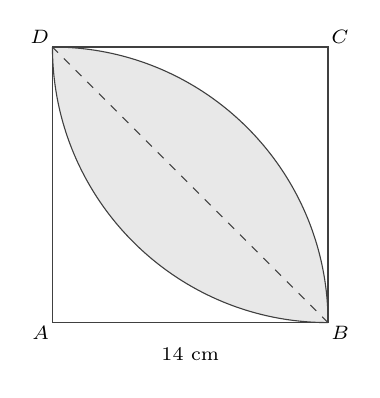
\begin{tikzpicture}[fig,every node/.style={font=\scriptsize}]
\fill[figfill] (3.5,0) arc (0:90:3.5) arc (180:270:3.5) -- cycle;
\draw[fig] (0,0) rectangle (3.5,3.5);
\draw[fig] (3.5,0) arc (0:90:3.5);
\draw[fig] (0,3.5) arc (180:270:3.5);
\draw[fig,dashed] (3.5,0) -- (0,3.5);
\node[below left,inner sep=1pt] at (0,0) {$A$};
\node[below right,inner sep=1pt] at (3.5,0) {$B$};
\node[above right,inner sep=1pt] at (3.5,3.5) {$C$};
\node[above left,inner sep=1pt] at (0,3.5) {$D$};
\node[below] at (1.75,-0.20) {$14$~cm};
\end{tikzpicture}
\end{center}
\end{answerblock}

\Needspace{16\baselineskip}
\ques A square garden has side $28$~m. At each corner there is a flower bed shaped like a quarter circle of radius $14$~m, with its centre at the corner of the garden. The rest of the garden is lawn.\par
\pc{a}{Find the area of the lawn.}
\pc{b}{Find the perimeter of the lawn.}
\pc{c}{The gardener makes the flower beds smaller, with radius $7$~m. Find the new area of the lawn and the new perimeter of the lawn.}
\pc{d}{Did the perimeter of the lawn increase or decrease in (c)? Explain why.}
\begin{center}
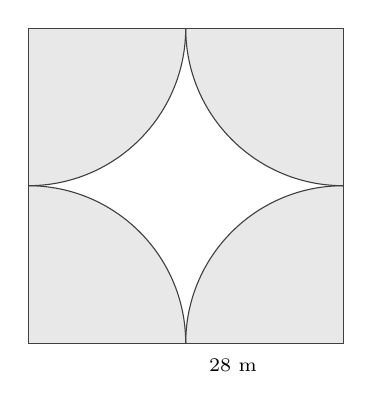
\begin{tikzpicture}[fig,every node/.style={font=\scriptsize}]
\fill[figfill] (0,0) -- (2,0) arc (0:90:2) -- cycle;
\fill[figfill] (4,0) -- (2,0) arc (180:90:2) -- cycle;
\fill[figfill] (4,4) -- (4,2) arc (270:180:2) -- cycle;
\fill[figfill] (0,4) -- (0,2) arc (270:360:2) -- cycle;
\draw[fig] (0,0) rectangle (4,4);
\draw[fig] (2,0) arc (0:90:2);
\draw[fig] (2,0) arc (180:90:2);
\draw[fig] (4,2) arc (270:180:2);
\draw[fig] (0,2) arc (270:360:2);
\node[below] at (2.6,-0.08) {$28$~m};
\end{tikzpicture}
\end{center}
\begin{answerblock}
\ap{a} The four quarter circles make one full circle of radius $14$~m.\nl
Beds $=\dfrac{22}{7}\times14\times14=616$~m$^2$, so the lawn $=28\times28-616=784-616=168$~m$^2$.
\ap{b} The boundary of the lawn is made of four quarter arcs, which make one full circumference.\nl
Perimeter $=2\times\dfrac{22}{7}\times14=88$~m.
\ap{c} With radius $7$~m the beds make one circle of area $\dfrac{22}{7}\times7\times7=154$~m$^2$.\nl
Lawn $=784-154=630$~m$^2$. Perimeter $=2\times\dfrac{22}{7}\times7=44$~m of arcs, plus four straight pieces of $28-7-7=14$~m each, so $44+4\times14=100$~m.
\ap{d} The perimeter increased, because $100$~m is more than $88$~m.\nl
With radius $14$~m the beds touch at the midpoints of the sides, so the boundary of the lawn is only arcs. With radius $7$~m the arcs are shorter, but four straight pieces appear along the sides of the square.
\begin{center}
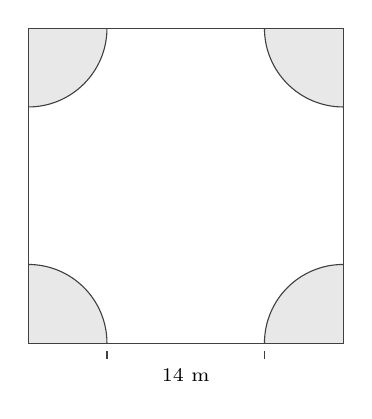
\begin{tikzpicture}[fig,every node/.style={font=\scriptsize}]
\fill[figfill] (0,0) -- (1,0) arc (0:90:1) -- cycle;
\fill[figfill] (4,0) -- (3,0) arc (180:90:1) -- cycle;
\fill[figfill] (4,4) -- (4,3) arc (270:180:1) -- cycle;
\fill[figfill] (0,4) -- (0,3) arc (270:360:1) -- cycle;
\draw[fig] (0,0) rectangle (4,4);
\draw[fig] (1,0) arc (0:90:1);
\draw[fig] (3,0) arc (180:90:1);
\draw[fig] (4,3) arc (270:180:1);
\draw[fig] (0,3) arc (270:360:1);
\draw[fig] (1,-0.10) -- (1,-0.20);
\draw[fig] (3,-0.10) -- (3,-0.20);
\node[below] at (2,-0.20) {$14$~m};
\end{tikzpicture}
\end{center}
\end{answerblock}
\end{document}
